% !TeX spellcheck = en_US

%
% FH Technikum Wien
% !TEX encoding = UTF-8 Unicode
%
% Erstellung von Master- und Bachelorarbeiten an der FH Technikum Wien mit Hilfe von LaTeX und der Klasse TWBOOK
%
% Um ein eigenes Dokument zu erstellen, müssen Sie folgendes ergänzen:
% 1) Mit \documentclass[..] einstellen: Master- oder Bachelorarbeit, Studiengang und Sprache
% 2) Mit \newcommand{\FHTWCitationType}.. Zitierstandard festlegen (wird in der Regel vom Studiengang vorgegeben - bitte erfragen)
% 3) Deckblatt, Kurzfassung, etc. ausfüllen
% 4) und die Arbeit schreiben (die verwendeten Literaturquellen in Literatur.bib eintragen)
%
% Getestet mit TeXstudio mit Zeichenkodierung ISO-8859-1 (=ansinew/latin1) und MikTex unter Windows
% Zu beachten ist, dass die Kodierung der Datei mit der Kodierung des paketes inputenc zusammen passt!
% Die Kodierung der Datei twbook.cls MUSS ANSI betragen!
% Bei der Verwendung von UTF8 muss dnicht nur die Kodierung des Dokuments auf UTF8 gestellt sein, sondern auch die des BibTex-Files!
%
% Bugreports und Feedback bitte per E-Mail an latex@technikum-wien.at
%
% Versionen
% *) V0.7: 9.1.2015, RO: Modeline angepasst und verschoben
% *) V0.6: 10.10.2014, RO: Weitere Anpassung an die UK
% *) V0.5: 8.8.2014, WK: Literaturquellen überarbeitet und angepasst
% *) V0.4: 4.8.2014, WK: Initalversion in SVN eingespielt
%
\documentclass[MGS,Master,english]{twbook}%\documentclass[Bachelor,BMR,german]{twbook}
\usepackage[utf8]{inputenc}
\usepackage[T1]{fontenc}
\usepackage{graphicx}
%\usepackage[disable]{todonotes} % notes not showed
\usepackage[draft]{todonotes} % notes showed

%
% Bitte in der folgenden Zeile den Zitierstandard festlegen
\newcommand{\FHTWCitationType}{HARVARD} % IEEE oder HARVARD möglich - wenn Sie zwischen IEEE und HARVARD wechseln, bitte die temorären Dateien (aux, bbl, ...) löschen
%
\ifthenelse{\equal{\FHTWCitationType}{HARVARD}}{\usepackage{harvard}}{\usepackage{bibgerm}}

% Definition Code-Listings Formatierung:
\usepackage[final]{listings}
\lstset{captionpos=b, numberbychapter=false,caption=\lstname,frame=single, numbers=left, stepnumber=1, numbersep=2pt, xleftmargin=15pt, framexleftmargin=15pt, numberstyle=\tiny, tabsize=3, columns=fixed, basicstyle={\fontfamily{pcr}\selectfont\footnotesize}, keywordstyle=\bfseries, commentstyle={\color[gray]{0.33}\itshape}, stringstyle=\color[gray]{0.25}, breaklines, breakatwhitespace, breakautoindent}
\lstloadlanguages{[ANSI]C, C++, [gnu]make, gnuplot, Matlab}

%Formatieren des Quellcodeverzeichnisses
\makeatletter
% Setzen der Bezeichnungen für das Quellcodeverzeichnis/Abkürzungsverzeichnis in Abhängigkeit von der eingestellten Sprache
\providecommand\listacroname{}
\@ifclasswith{twbook}{english}
{%
    \renewcommand\lstlistingname{Code}
    \renewcommand\lstlistlistingname{List of Code}
    \renewcommand\listacroname{List of Abbreviations}
}{%
    \renewcommand\lstlistingname{Quellcode}
    \renewcommand\lstlistlistingname{Quellcodeverzeichnis}
    \renewcommand\listacroname{Abkürzungsverzeichnis}
}
% Wenn die Option listof=entryprefix gewählt wurde, Definition des Entyprefixes für das Quellcodeverzeichnis. Definition des Macros listoflolentryname analog zu listoflofentryname und listoflotentryname der KOMA-Klasse
\@ifclasswith{scrbook}{listof=entryprefix}
{%
    \newcommand\listoflolentryname\lstlistingname{}
}{%
}
\makeatother
\newcommand{\listofcode}{\phantomsection\lstlistoflistings}

%
% Einträge für Deckblatt, Kurzfassung, etc.
%
\title{Using Procedural Content Generation via Machine Learning as a Game Mechanic}
\author{Bernhard Rieder, BSc}
\studentnumber{1610585006}
%\author{Titel Vorname Name, Titel\and{}Titel Vorname Name, Titel}
%\studentnumber{XXXXXXXXXXXXXXX\and{}XXXXXXXXXXXXXXX}
\supervisor{Dipl.-Ing. (FH) Alexander Hofmann}
%\supervisor[Begutachter]{Titel Vorname Name, Titel}
%\supervisor[Begutachterin]{Titel Vorname Name, Titel}
\secondsupervisor{Dr. Jichen Zhu \and{} Dr. Santiago Onta\~{n}\'{o}n}
%\secondsupervisor[Begutachter]{Titel Vorname Name, Titel}
%\secondsupervisor[Begutachterinnen]{Titel Vorname Name, Titel}
\place{Philadelphia}
\kurzfassung{Blah blah blah, das ist meine Kurzfassung über die Verwendung von Prozeduraler Inhaltsgenerierung mit Machine Learning als eine Spielmechanik, blah blah blah}
\schlagworte{Prozedurale Inhaltsgenerierung, Machine Learning, Spielemechanik, Künstliche Intelligenz, Spieleentwicklung}
\outline{
	Blah blah blah, this is my outline about the use of procedural content generation via machine learning as a game mechanic, blah blah blah\\
	\\
	\textit{Procedural Content Generation (PCG) is an essential topic in modern games. Notably, it is a very crucial topic for independent game developers due to a low budget, where PCG can generate much content for less effort. As the importance of PCG for game development increases, researchers explore new avenues for generating high-quality content with or without human involvement. Here is where Machine Learning comes into play and extends the capabilities of PCG. Procedural Content	Generation via Machine Learning (PCGML) systems can be trained on its own and evolve if they do not generate usable output and offer a broad application possibility. One promising way of using PCGML is the use as a game mechanic. Therefore, this research will address and focus on the possibilities and development process of how PCGML can be used as a game mechanic and is going to provide a firrst demonstration of its use.}\\
	\\
	Abstracts can vary in length from one paragraph to several pages, but they follow the IMRaD format and
	typically spend:
	\begin{itemize}
		\item 25\% of their space on importance of research (Introduction)
		\item 25\% of their space on what you did (Methods)
		\item 35\% of their space on what you found: this is the most important part of the abstract (Results)
		\item 15\% of their space on the implications of the research (Discussion)
	\end{itemize}
}
\keywords{Procedural Content Generation, Machine Learning, Game Mechanic, Artifial Intelligence, Game Development}
\acknowledgements{Many thanks to mr Alexander Hofmann who gave me the possibilty to write my master thesis abroad at the Drexel University. Also many thanks to the Drexel University and Dr. Michael Wagner who gave me the opportunity to be a part of their team while i was writing my master thesis there. Lastly, many thanks to Dr. Santiago Ontanon and Dr. Jichen Zhu who supported me, ....}

\begin{document}
%Festlegungen für den HARVARD-Zitierstandard
\ifthenelse{\equal{\FHTWCitationType}{HARVARD}}{
\bibliographystyle{Harvard_FHTW_MR}%Zitierstandard FH Technikum Wien, Studiengang Mechatronik/Robotik, Version 1.2e
\citationstyle{dcu}%Correct citation-style (Harvardand, ";" between citations, "," between author and year)
\citationmode{abbr}%use "et al." with first citation
\iflanguage{ngerman}{
    %Deutsch Neue Rechtschreibung
    \newcommand{\citepic}[1]{(Quelle: \protect\cite{#1})}%Zitat: Bild
    \newcommand{\citefig}[2]{(Quelle: \protect\cite{#1}, S. #2)}%Zitat: Bild aus Dokument
    \newcommand{\citefigm}[2]{(Quelle: modifiziert "ubernommen aus \protect\cite{#1}, S. #2)}%Zitat: modifiziertes Bild aus Dokument
    \newcommand{\citep}{\citeasnoun}%In-Line Zitiat entweder mit \citep{} oder \citeasnoun{}
    \newcommand{\acessedthrough}{Verf{\"u}gbar unter:}%Für URL-Angabe
    \newcommand{\acessedthroughp}{Verf{\"u}gbar bei:}%Für URL-Angabe (Geschützte Datenbank, Zugriff durch FH)
    \newcommand{\acessedat}{Zugang am}%Für URL-Datum-Angabe
    \newcommand{\singlepage}{S.}%Für Seitenangabe (einzelne Seite)
    \newcommand{\multiplepages}{S.}%Für Seitenangabe (mehrere Seiten)
    \newcommand{\chapternr}{K.}%Für Kapitelangabe
    \renewcommand{\harvardand}{\&}%Harvardand in Zitaten
    \newcommand{\abstractonly}{ausschließlich Abstract}
    \newcommand{\edition}{. Auflage}%Angabe der Auflage
}{
\iflanguage{german}{
    %Deutsch
    \newcommand{\citepic}[1]{(Quelle: \protect\cite{#1})}%Zitat: Bild
    \newcommand{\citefig}[2]{(Quelle: \protect\cite{#1}, S. #2)}%Zitat: Bild aus Dokument
    \newcommand{\citefigm}[2]{(Quelle: modifiziert "ubernommen aus \protect\cite{#1}, S. #2)}%Zitat: modifiziertes Bild aus Dokument
    \newcommand{\citep}{\citeasnoun}%In-Line Zitiat entweder mit \citep{} oder \citeasnoun{}
    \newcommand{\acessedthrough}{Verf{\"u}gbar unter:}%Für URL-Angabe
    \newcommand{\acessedthroughp}{Verf{\"u}gbar bei:}%Für URL-Angabe (Geschützte Datenbank, Zugriff durch FH)
    \newcommand{\acessedat}{Zugang am}%Für URL-Datum-Angabe
    \newcommand{\singlepage}{S.}%Für Seitenangabe (einzelne Seite)
    \newcommand{\multiplepages}{S.}%Für Seitenangabe (mehrere Seiten)
    \newcommand{\chapternr}{K.}%Für Kapitelangabe
    \renewcommand{\harvardand}{\&}%Harvardand in Zitaten
    \newcommand{\abstractonly}{ausschließlich Abstract}
    \newcommand{\edition}{. Auflage}%Angabe der Auflage
}{
    %Englisch
    \newcommand{\citepic}[1]{(Source: \protect\cite{#1})}%Zitat: Bild
    \newcommand{\citefig}[2]{(Source: \protect\cite{#1}, p. #2)}%Zitat: Bild aus Dokument
    \newcommand{\citefigm}[2]{(Source: taken with modification from \protect\cite{#1}, p. #2)}%Zitat: modifiziertes Bild aus Dokument
    \newcommand{\citep}{\citeasnoun}%In-Line Zitiat entweder mit \citep{} oder \citeasnoun{}
    \newcommand{\acessedthrough}{Available at:}%Für URL-Angabe
    \newcommand{\acessedthroughp}{Available through:}%Für URL-Angabe (Geschützte Datenbank, Zugriff durch FH)
    \newcommand{\acessedat}{Accessed}%Für URL-Datum-Angabe
    \newcommand{\singlepage}{p.}%Für Seitenangabe (einzelne Seite)
    \newcommand{\multiplepages}{pp.}%Für Seitenangabe (mehrere Seiten)
    \newcommand{\chapternr}{Ch.}%Für Kapitelangabe
    \renewcommand{\harvardand}{\&}%Harvardand in Zitaten
    \newcommand{\abstractonly}{Abstract only}
    \newcommand{\edition}{~edition}%Edition -> note, that you have to write "edition = {2nd},"!
}}}

\maketitle

%
% .. und hier beginnt die eigentliche Arbeit. Viel Erfolg beim Verfassen!
%
\chapter{Introduction}
\ac{PCG} is an essential and aspiring topic in modern games and is extensively used for decades \cite{pcg::whatIsPCG}. Therefore, further research on different kinds of \ac{PCG} is necessary to provide new exciting techniques for games development. Notably, it is especially a very crucial topic for small independent game developer studios due to a low budget, where \ac{PCG} can generate much content for less effort and human resources \cite{pcg::shortHistoryOfDynamicAndPCG}. With this in mind, more and more storage will be available on a \ac{PC} or console in the future according to Moore's Law, and it is getting hard to design a various range of content in a short amount of time. While gamer and players will be getting used to massive amounts of content because of big gaming companies which can establish a broad range of new content without the use of PCG, the small development teams will not keep up as smooth as the market leaders. Here is where \ac{ML} comes into play. \ac{PCG} is getting much more accessible and powerful with the help of ML which combined form the new impressive technique of \ac{PCGML} \cite{pcgml::paper}.\\
A \ac{PCGML} system opens a lot of new possibilities due to the fact that it uses machine learning. For example, it can be trained on its own and evolve if they do not generate usable output \cite{pcgml::paper}. Furthermore, the system could also be trained by some designers with unique input or by a regular user with their creative input \cite{pcgml::paper}. \ac{PCGML} can be used for so many aspects of a game since it can learn from simple examples and instructions. Most current work on PCGML focuses on creating designed content like unlimited amounts of unique levels \cite{pcgml::paper}. But there are some open problems which needs to be addressed to utilize the whole power of PCGML. For this reason, one of an open problem is the use of \ac{PCGML} as a game mechanic which is a promising approach for evolving the overall player experience in games, which could guide the games industry and development into a new future of content acquisition \cite{pcgml::paper}.

\section{Idea}
\ac{PCGML} is a relatively new method and technique for creating different kinds of content in modern video games  for \ac{PC}, gaming consoles up to mobile devices. Most current work focuses mainly on replicating designed content to provide the player with infinite and unique variations on gameplay \cite{pcgml::paper}. Another great and innovative possible use of PCGML is its use as the main mechanic of a game, e.g. presenting the \ac{PCGML} system as an adversary or toy for the player to engage with \cite{pcgml::paper}. \\
The paradigm of using \ac{PCGML} as a game mechanic is a relevant and promising topic which is not addressed by now \cite{pcgml::paper}. Therefore, it needs detailed analysis on how it could be used best in games. For example, design of mechanics could include enticing the player to generate content that is significantly similar to or different from the corpus the system was trained on, or identify content examples that are outliers or typical examples of the system \cite{pcgml::paper}. Or players could also train \ac{PCGML} systems to generate examples that possess certain qualities or fulfill certain objective functions, teaching the player to operate a model by feeding it examples that shape its output in one direction or the other \cite{pcgml::paper}. \\ 
Treanor et al. \cite{ai::aiBasedGameDesignPattern} illustrated the following various design patterns for developing a game mechanic with \ac{AI} which could be used for an exemplary PCGML system: "\ac{AI} as Role-Model", "Trainee", "Editable", "Guided", "Co-Creator", "Adversary" or "Spectacle". Everyone of them provide a great guiding principle for designing and implementing a PCGML game mechanic.

\subsection{Advantages}
As already mentioned, PCGML can offer an unlimited amount of content when is comes to designed content generation which is also applicable for game mechanics. There is a good amount of replay value with PCG mechanics in general due to the fact of procedural generation itself but with the help of ML this is going to increase significantly. For example, players could play a game e.g. 10 times and experience different ways of fulfilling objectives every time. In particular, players could also emerge emotional feelings for a PCGML system which is used as a trainee and remains throughout the whole game. Hence, this could create positive and magnificent memories for the players and thus for the game experience and the game itself.

\subsection{Challenges}
One of the major challenges in creating a PCGML game mechanic is the design of the mechanic which should fulfill some crucial requirements of game design to offer a good player experience. As well, the machine learning part is going to be a challenging part since it might take a lot of tweaking to get a fully working AI algorithm.

\section{Desired Goals}
It is important to note that the main idea of this master thesis is to create game mechanics which rely on the principles of PCGML rather than creating a generic PCGML game mechanic generator.\\
With this in mind, it is expected to provide a first insight in the use of \ac{PCGML} as a game mechanic in modern games. The primary goal is to demonstrate the possibilities as well as the development process of game mechanics when it comes to the use of \ac{PCGML} and also how games should work when using \ac{PCGML}.\\
Additionally, there are some further questions which need to be addressed by this thesis. It should impart some theoretical and practical knowledge of PCG, ML, \ac{PCGML}, and \ac{PCGML} as a game mechanic. Talking about theoretical and practical knowledge which means that it should show how these concepts are going to be implemented from scratch and which dependencies are given and needed for a fully working implementation. \\
Furthermore, it should provide a good overview and function as a primer for developing proprietary \ac{PCGML} game mechanics in a specific game engine or other environments. Especially, a focus on implementations in commonly used game engines is desired since most of the independent game developers are using game engines instead of creating their own engine because that is often a long process of development. \\
A substantial goal for this work is a fully working game with \ac{PCGML} as the core game mechanic which acts as a perfect example of what is possible with this kind of functionality. It is considered to playtest the game by different kinds of people where every feedback and idea will be evaluated to increase the usability of the \ac{PCGML} game mechanics. Also, since video games in general are performance-heavy applications, it should cover a performance report as a point of reference for future implementations and uses. As an additional point, it should include an outlook of the opportunities of \ac{PCGML} game mechanics in future games and work, which should also function as motivation for future work in this field of research.\\
Generally speaking, it should be an overall guideline for bringing \ac{PCGML} game mechanics into a game.

\section{Proceedings}
\subsection{Approach}
As said before, one goal of this thesis shall be the support of small and independent game developers with an introduction into PCGML game mechanics in a game engine like Unreal Engine or Unity. For doing so, it is going to address all important topics which are dependent on building PCGML game mechanics and their use in game engines. It is attempted to start with the central fields of interest like game mechanics, PCG and ML to create awareness for this topics in the a beginning. Afterwards, all the beforehand discussed topics shall be combined into PCGML and furthermore into PCGML game mechanics. In particular, theoretical usage is not only the most important subject which is the reason for providing at least some conceptual implementations on PCG, ML and PCGML. The implementation of a PCGML game mechanic with subsequent playtests as an evaluation of the concepts is also a necessary matter which should complete the introduction.

\subsection{Agenda}
The agenda will be split into two parts. The first one is a scientific-informal part about getting to know more about the foundation of \ac{PCGML} and its use as a game mechanic. Since \ac{PCGML} is a relatively new theme in game development, it focuses on topics regarding core knowledge of \ac{PCG} and \ac{ML} separately and game mechanics to act as a base for further research on \ac{PCGML} as a game mechanic. Following topics shall be a part of the informal research:
\begin{itemize}
	\item Game mechanics and their use in games.
	\item Necessary and important theory of PCG and ML which is dependent for PCGML with a constant focus on game mechanics, like types of PCG and some of the most used learning and training models of ML.
	\item The conceptual use of PCG and ML in a game engine as well as best practices, other approaches and possible issues when using PCG and ML in games and a game engine.
	\item Overview of possible game mechanics with \ac{PCGML}.
\end{itemize}
The second part of the agenda deals with the central scientific problem of this master thesis. It addresses every aspect of \ac{PCGML} and discusses how to use \ac{PCGML} as a game mechanic in modern games with a focus on the maximum possible benefit for game developers. This part shall contain the following fields of research: 
\begin{itemize}
	\item Theory of \ac{PCGML} and its methods in general.
	\item Research on different \ac{PCGML} implementations and practical usage possibilities in a game engine.
	\item Comparison of \ac{PCGML} methods regarding their use in \ac{PCGML} as a game mechanic.
%	\item Comparison of \ac{PCGML} learning models.
%	\item Evaluation of \ac{PCGML} hardware and software requirements.
	\item Conceptual implementation of possible \ac{PCGML} game mechanics in a game engine and subsequent evaluation as well as a detailed comparison.
	\item Development of a game with one of the best-evaluated \ac{PCGML} game mechanic as the central game mechanic of the game.
	\item Proof of concept with playtest sessions and evaluation of its feedback.
	\item Research summary with meaning of \ac{PCGML} as a game mechanic for the future of games. 
\end{itemize}

\subsection{Methodological Considerations}
Just as important as the agenda are some methodological questions which need to be raised and answered at both research and implementation time, like:
\begin{itemize}
	\item Which \ac{PCGML} techniques are best for a game? Or which learning and training models for \ac{PCGML} have the greatest advantage?
	\item Which programming languages fit best for the use with \ac{PCGML} in conjunction with a game engine and which game engine should be used? 
	\item Is it better to use an online or offline version of \ac{PCGML}? Related to this field is the question of requirements on hardware and software regarding \ac{PCGML} as well if multithreading needs to be minded.
	\item Which game mechanics could be implemented in \ac{PCGML} and suits a game?
	\item What evaluation criteria shall be used for the playtesting session?
\end{itemize} 


\section{Thesis Overview}
Finish and write this section afterwards the thesis is finished!

\section{Target Group}
This thesis is dedicated to advanced game developers who are interested in using PCGML game mechanics in their game. The theoretical part assumes a basic knowledge of game design and mechanics, PCG and ML since it will not be explained everything in detail. In particular, specific topics of PCG and ML which contribute to the use of PCGML as a game mechanic will be discussed and handled in more detail.\\
The practical part concentrates primarily on programming in different programming languages like C++ which makes it necessary for the reader to be familiar with programming. Special algorithms used thorough the chapters will be covered in detail whereas basic algorithm knowledge is assumed. Furthermore, it does not require special game development back-end skills since it addresses the use of the technique in game engines.

%
% ------------------------------- NEW CHAPTER ------------------------------- %
%
\clearpage
\chapter{Game Mechanics}
Starting this chapter with a quick insight on the \ac{MDA} framework which was introduced by \cite{mechanic::MDA}, helps to understand the foundation and the correlation of game mechanics in video games. In general, the MDA framework describes the division of gaming experience emergence into three dependent parts, starting with "Rules" followed by "System" and concluded with "Fun" \cite{mechanic::MDA}. These fundamental parts can be represented by the designs of "Mechanics", "Dynamics" and "Aesthetics" in a game  \cite{mechanic::MDA}. Therefore, a large amount of gaming experience is made out of mechanics and a game will not be fun at all if their mechanics are not properly thought through even if it has amazing graphics \cite{gameDesign::gameMechanicsAdvancedGameDesign}. Consequently, game mechanics are acting as one of the most important roles in game design which is the reason to create awareness for this topic in the beginning of the thesis.  
% one could mention the DDE framwork besides MDA \cite{mechanic::fromMdaToDde}

\section{Definition}
As already indicated, a game mechanic is a main concept with many underlying sub-concepts like dynamics, aesthetics, rules, systems, processes, procedures or data which all characterize the heart of a game besides story and technology \cite{gameDesign::gameMechanicsAdvancedGameDesign} \cite{gameDesign::bookOfLenses}. It also creates gameplay and the experience of playing a game. But besides, there is no concrete definition of what a game mechanic is. Nonetheless, there are some key concepts mentioned by different game designers which contribute to an interpretation of what a game mechanic can or shall be or do:
\begin{itemize}
	\item Defines how a game is played, their objectives can be achieved or how to lose a game. Thus, mechanics are precisely designed, detailed, specified and implemented to fulfill playability. \cite{gameDesign::gameMechanicsAdvancedGameDesign} \cite{gameDesign::bookOfLenses}
	\item Often used to indicate the most influential and affecting aspect of a game which is also mostly referred as core mechanic. \cite{gameDesign::gameMechanicsAdvancedGameDesign}
	\item Enables interaction and control of game objects and elements. \cite{gameDesign::gameMechanicsAdvancedGameDesign}
	\item Mostly hidden from the player, media-independent and easy to learn. For example, rules are more considered as printed and players are aware of them because they can see or read them whereby mechanics like an enemy damage model with its damage points are hidden. \cite{gameDesign::gameMechanicsAdvancedGameDesign}
	\item A game mechanic can also be seen as a meeting point for a designers question and their provided tools for answering that question by a player. \cite{mechanic::gamasutra::MikeStout}
\end{itemize}

\section{Types of Mechanics}
It is obvious that one tries to divide possible mechanics into concrete types since of their various possibilities and shared base ideas. For this purpose, \cite{gameDesign::gameMechanicsAdvancedGameDesign} summarized different types of game mechanics which are mainly used in games nowadays. They first categorized them into the following five types which are listed below with some related mechanics:
\begin{itemize}
	\item \textbf{Physics}: Motion and forces like gravity, shooting, fighting, jumping, moving, driving or any other kind of position change. \cite{gameDesign::gameMechanicsAdvancedGameDesign}
	\item \textbf{Internal Economy}: In general, all game elements which involve transaction like collecting, consuming, harvesting, buying, building, upgrading, risking or customizing of resources like currency, ammunition, portions, power ups or other kind of items. Also the use of energy, health, lives, power, points, popularity or experience and management actions for team, resources or inventory. \cite{gameDesign::gameMechanicsAdvancedGameDesign}
	\item \textbf{Progression Mechanisms}: Usually the elements or mechanisms which are controlling the players progress in the game world. For example, quests, missions, competitions, tournaments, races, challenges, levers, switches, locks, keys or special items which allow a player to defeat an AI. \cite{gameDesign::gameMechanicsAdvancedGameDesign}
	\item \textbf{Tactical Maneuvering}: Is mainly used in strategy games but also in roleplay or simulation games and often deals with the placement of elements on a map like in chess. Mechanics are for instance internal tactics where a player gains offensive or defensive advantage, also team tactics and management of resources and buildings. \cite{gameDesign::gameMechanicsAdvancedGameDesign}
	\item \textbf{Social Interaction}: Refer to rules that govern play-acting of a player or strategic actions of forming allies to defeat bosses or other allies like in roleplay games. Further mechanics would be e.g. reward of giving gifts, inviting new friends to join the game, competition between players or in particular mechanics in a co-op game where at least two players are forced to work together to achieve an objective. \cite{gameDesign::gameMechanicsAdvancedGameDesign}
\end{itemize}
In addition, all prior mentioned mechanics can be subdivided into discrete and continuous mechanics in terms of their internal values \cite{gameDesign::gameMechanicsAdvancedGameDesign}. For example, internal economy is mostly discrete since it is mostly represented by a simple integer value because e.g. a player cannot pick up half of a portion — either the portion is picked up completely or not \cite{gameDesign::gameMechanicsAdvancedGameDesign}. In contrast, continuous mechanics make use of high precision values for accuracy and is continuously calculated throughout the game like the movement of a character \cite{gameDesign::gameMechanicsAdvancedGameDesign}. \\
Furthermore, every type can also be used to categorize game genres in which they are used the most. The distinction can be seen in table \ref{GameMechanicsToGenre}.
\begin{table}[!htbp]
	\centering
	\resizebox{\textwidth}{!}
	{%
		\begin{tabular}{l||c|c|c|c|c|}
			\cline{2-6}
			& \multicolumn{5}{c|}{\textbf{Game Mechanics}}        \\ \hline 
			\multicolumn{1}{|l||}{\textbf{Game Genres}}  & Physics & Economy & Progression & Tactical & Social \\ \hline \hline
			\multicolumn{1}{|l||}{Action}                & x       & x       & x           &          &        \\ \hline
			\multicolumn{1}{|l||}{Strategy}              & x       & x       & x           & x        & x      \\ \hline
			\multicolumn{1}{|l||}{Roleplay}              & x       & x       & x           & x        & x      \\ \hline
			\multicolumn{1}{|l||}{Sports}                & x       & x       & x           & x        &        \\ \hline
			\multicolumn{1}{|l||}{Vehicle Simulation}    & x       & x       & x           &          &        \\ \hline
			\multicolumn{1}{|l||}{Management Simulation} &         & x       & x           & x        & x      \\ \hline
			\multicolumn{1}{|l||}{Adventure}             &         & x       & x           &          &        \\ \hline
			\multicolumn{1}{|l||}{Puzzle}                & x       &         & x           &          &        \\ \hline
			\multicolumn{1}{|l||}{Social Games}          &         & x       & x           &          & x      \\ \hline
		\end{tabular}%
	}
	\caption{Game Genres and their related Game Mechanics \protect\cite{gameDesign::gameMechanicsAdvancedGameDesign}}
	\label{GameMechanicsToGenre}
\end{table}\\
But since the overview of \cite{gameDesign::gameMechanicsAdvancedGameDesign} is no universal taxonomy for game mechanics, there is another great approach to categorize them as described by \cite{gameDesign::bookOfLenses}. Following rather similar types to \cite{gameDesign::gameMechanicsAdvancedGameDesign}'s approach are used which also correlate to some parts described in the MDA framework:
\begin{itemize}
	\item \textbf{Space}: Every game takes places in some kind of game spaces. Spaces can be continuous or discrete, consists of dimensions and can have bounded areas that may or may not be connected. The mechanics of Tic-Tac-Toe are a good example for this kind of mechanics which are taking place in a discrete space. \cite{gameDesign::bookOfLenses}
	\item \textbf{Time}: Contains mechanics which are using time, clocks, races or controlled time. A popular example for this kind of mechanics is the game Superhot which tweaks the time to create a unique game experience. \cite{gameDesign::bookOfLenses}
	\item \textbf{Objects, Attributes, States and Actions}: If these terms are compared to the structural elements of a sentence then the game objects represent the nouns, attributes and states are their adjectives and actions are the verbs of a game mechanic. This paradigm represents most of the mechanics which are used for interaction with game elements. \cite{gameDesign::bookOfLenses}
	\item \textbf{Rules}: Combines all spaces, times, objects, actions and their consequences, constraints and the goals to form the behavior of the game. \cite{gameDesign::bookOfLenses}
	\item \textbf{Skill}: Shifts the focus to the players and focus on their physical, mental and social skills. That means it includes mechanics like dexterity, coordination, memory, observation, puzzle solving, reading or fooling an opponent or coordinating with teammates .  \cite{gameDesign::bookOfLenses}
\end{itemize}

%\section{Mechanics in Popular Games}
%"mechanics of monopoly -> prices of all the properties, text of all the chance and community chest cards - in other words, everything that affects the operation of the game."
%\subsection{Tetris}
%...

\section{Considerations with \acl{PCG} and \acl{ML}} \label{mechanicsConsiderationsPCGandML}
This chapter shall state some crucial considerations for the next chapters since \ac{PCG} and \ac{ML} game mechanics are not visible used in big game titles and therefore need some special attention on their implementation in a game. One of the good things is that there are dozens of possibilities for mechanics which should not create a big problem in coming up with new and novel ideas for new mechanics. With certainty, the focus of implementing such mechanics will lie on the introduction to the player and their ability for interactions due to the fact that PCG and ML mechanics could confuse some players. Therefore, the implemented mechanics should kept as easy as possible if user interaction is needed instead of creating complex but novel and unusual mechanics. A good starting point is to design the mechanics as soon as the main gameplay concept is set and adhere to the design stages of concept, elaboration and tuning during development \cite{gameDesign::gameMechanicsAdvancedGameDesign}.\\
It is necessary to list some possible design flaws which need to be avoided since game mechanics shall amaze people instead of frustrate them during playing a game. In addition, a lot of detailed planning is made to come up with new extraordinary mechanics where plans about their proper introduction are missing \cite{mechanic::gamasutra::MaxPears}. For this reason, it is relevant to address some common mistakes and their possible improvements:
\begin{itemize}
	\item Do not introduce all mechanics of a game as fast as possible because players need time to learn and get used to mechanics. For this reason, just introduce one mechanic at a time! \cite{mechanic::gamasutra::MaxPears}
	\item Do not introduce mechanics when the player has no time to explore them. They need time in their own pace to explore the mechanics otherwise they will not enjoy their new ability. \cite{mechanic::gamasutra::MaxPears}
	\item Use and create feedback loops for game mechanics otherwise players will not know what to do with them. For example, if someone uses a portion and there is no obvious visualization for the use of it then the player does not know for what to use it. \cite{gameDesign::gameMechanicsAdvancedGameDesign}\\
	Sometimes feedback is one of the most important elements which can be seen in the concept of the basic grammar model introduced by \cite{mechanic::BasicGrammarModel}. This model can be applied to most of popular games. It loops the concepts of a mental model, intent, input, actual model and rules, state change and feedback \cite{mechanic::BasicGrammarModel}. Where the mental model of a player assumes how a game works and what their intentions for the input and the actual input does, what then really happens with their input in terms of applying core mechanics, concluded with a feedback for their inputs \cite{mechanic::BasicGrammarModel}. If no feedback would be given then the player could never update their mental model and cannot progress through a game. Feedback can be given in a simple binary or even complex way \cite{mechanic::BasicGrammarModel}.
	\item Besides feedback loops, do not forget to provide the player with directions for parts of your mechanic which are or could not be obvious \cite{mechanic::gamasutra::MaxPears}. Further tutorials should be easily accessible if they are needed because there is nothing more frustrating to a player than being confused \cite{mechanic::gamasutra::DanielDoan}.
	\item For core mechanics does apply: provide clear rules on how to be successful, create a natural interaction but do not forget to challenge the player and provide possibility for natural progression of their skills, properly guide the player towards successfully completing their in-game objectives with directions and feedback, allow the player to move naturally from objective to objective without the necessity of using the core mechanic and provide options besides the core mechanic. \cite{mechanic::gamasutra::DanielDoan}
	\item In general, the skill of a player will grow over throughout the game which means that the difficulty curve shall match the player's skill throughout a game. \cite{mechanic::gamasutra::DanielDoan}
	\item Like described by \cite{mechanic::generateAndAdaptingMechanics} where their goal was to generate and adapt game mechanics, it is necessary that mechanics fulfill the requirements of playability in order to create acceptable experience. For example, a requirement could be that it is necessary that a player can reach the end of a level or win a fight without dying. Overall, it should ensure that a game is playable to a specific given goal with that mechanic.
\end{itemize} 


%
% ------------------------------- NEW CHAPTER ------------------------------- %
%
\clearpage
\chapter{\acl{PCG}}
This topic is a very big one which has evolved throughout the years and many research is done in \ac{PCG}. For this reason, it is a necessity to introduce the most common parts of PCG to understand the concepts and therefore be able to understand the further use in \ac{PCGML}.\\
The definition we will use is that PCG is the algorithmic creation of game content with limited or indirect user input [32]. In other words, PCG refers to computer software that can create game content on its own, or together with one or many human players or designers. \cite{pcg::whatIsPCG}
Like: a software tool that creates dungeons, weapons, ..; game engine middleware that rapidly populates a game world with vegatetion

\section{Introduction}
\cite{pcg::PCGinGameIndustry} Game content construction and generation are laborious and expensive. Procedural content generation (PCG) aims at generating game content automatically using algorithms, reducing the cost of game design and development.\\
Procedural content generation refers to the creation of game content automatically (or semi-automatically) through algorithmic means.\\
The results from the application of PCG algorithms can be all kinds of elements affecting the gameplay: terrain, maps, layers, stories, dialogues, quests, characters, rules, dynamics, or weapons.\\
\\
It would be futile to hope to come up with a definition of procedural content generation in games that everybody agrees on. PCG has been attempted by too many people with too many different perspectives for this to happen. A graphics researcher, a game designer in the industry and an academic working on artifcial intelligence techniques would be unlikely to agree even on what "content" is, and much less which generation techniques to consider interesting. We argue that PCG is a concept with fuzzy and unclear boundaries. Besides, exact definitions of concepts are commononly in mathematics. \cite{pcg::whatIsPCG}\\
\\
PCG has been used in games for many reasons, including addressing technical limitations, improving replayability, and providing infinite worlds for the player to explore. \cite{pcg::endlessWeb}\\
There are three major ways that PCG has traditionally been used in digital game design: to improve replayability, to resolve technical limitations, and to provide players with an environment to explore that is so vast it could not be created by human designers.\cite{pcg::endlessWeb}

\subsection{Reasons to Use}
There are many reason why to use PCG in games or other applications like research. For this reason, \cite{pcg::inGameDesign} came up with two classifications representing the motivation behind using PCG.
\subsubsection{Utilization}
The first one is utilization which is one of the main argument why PCG is popular. It can be time-saving because it could produce more content than a human in an hour like a whole galaxy in No Man's Sky \cite{noMansSky} which is in fact created by PCG, it overcomes technical limitations in terms of their use for devices with e.g. limited space like mobile devices, is expandable and has reusable code due to modularity and same field of applications and it increases replayability because it can generate many but different instances of a content \cite{pcg::inGameDesign}.

\subsubsection{Uniqueness}
Second argument why PCG is commonly used is the uniquness of their output. It offers an individual experiences with i.e. different generated content every time, creates new gameplay and interaction modes through replayability or possible player interaction, it is unpredictable which can be a thrilling fact for players but also designers, it can create bizarre content no human might think of and it can be an inspiration of infinity because of its possibility of infinitely creating content \cite{pcg::inGameDesign}.
\subsection{Types}
a pcg system is a generic term for any piece of software that does pcg and there are many different possible uses \cite{pcg::book}
methaphors for PCG in pcg book intro\\
\begin{itemize}
	\item as a tool: instruments that give designers enhanced capabilities, in the way that a programmer’s development	environment; aim to improve a designer’s workflow. A common example is a PCG-enhanced level editor.
	\item materials:  Others define new kinds of materials, allowing a designer to work in a new medium, the way stone, clay, and laser installations are different materials for an artist. create new generative materials that a game designer manipulates and sculpts to produce content. A popular commercial example is SpeedTree.
	\item designer itself: carrying out fully autonomous design of parts or even entire games, rather than assisting game designers. less interaction with the human designer, and	instead has ambitions of designing content all on its own. In the limit case, a PCG designer turns into a fully autonomous game generator that creates new games, usually in a specific genre.
	\item domain experts: carrying with them extensive knowledge of game design that can be used to critique or improve designs. Many systems can be viewed through more	than one of these lenses, though few will exhibit all of them equally. a slightly different kind of system, full of knowledge about games or players, and able to apply it to critique and modify content. Often it will apply that expertise by being part of a system that also serves as a tool or a designer. A domain expert may have purely formal knowledge of games, such as what makes a particular set of rules elegant [6]. Or it may have extensive knowledge of human players, being able to predict what people will do in a game, and what they will find challenging, fun, or boring.
\end{itemize}



\subsection{Taxonomy}\label{PcgTaxonomy}
There are many use cases for using procedural generated content for different kind of problems with different methods and approaches. This variety of PCG possibilities made it necessary to find distinctive features and create a taxonomy of PCG to highlight the differences and similarities between approaches \cite{pcg::book}. In fact, there are two different views for a taxonomy which were described by \cite{pcg::survey} and \cite{pcg::book}. The first and initial approach was created by \cite{pcg::survey} whereas the new one derived from \cite{pcg::survey}'s taxonomy was given by \cite{pcg::book}.\\
As an initial classification, \cite{pcg::survey} extracted the following four classes by analyzing all possibilities of PCG which they could think of:
\begin{itemize}
	\item \textbf{Game Bit}: Basic elements of a game that do not affect the players gameplay. For example, procedural generated textures, sounds, trees, fire, stones, mountains or clouds. \cite{pcg::survey}
	\item \textbf{Game Space}: Represents game environments and usually consist of different game bits. One can think of e.g. dungeons maps, whole planets with procedural generated terrain, lakes, rivers and many more. \cite{pcg::survey}
	\item \textbf{Game System}: Includes all game elements like ecosystems or other relations between game objects like rules or objectives. \cite{pcg::survey}
	\item \textbf{Game Scenario}: Like occurring events in games which could be e.g. an event in a generated storyboard, the history of a character, a concept of levels or a puzzle. \cite{pcg::survey}
\end{itemize}
Whereas \cite{pcg::book} extended their view of possibilites for PCG and came up with the following 13 classes:
\begin{itemize}
	\item \textbf{Online vs Offline}: Is about game elements or content which is generated during runtime as the player is playing the game versus predefined and or pre-generated content which is created before the start of a game \cite{pcg::book}. Like an interactive maze which is generated during runtime versus a procedural generated terrain which is used as the uniform environment of the game and does not affect the players playing experience in terms of processing during the game.
	\item \textbf{Necessary vs Optional}: Distinguishes content which is necessary or required to reach an objective in a game and content which does not need to fulfill this or other requirements \cite{pcg::book}. For example, a terrain could be necessary to finish the game whereas a generated texture is just an optional content.
	\item \textbf{Degree and Dimensions of Control}: Describes content which is controlled via adjustable parameter or a seed for the \ac{RNG}. In general, content where designers or users and players have control over the generation space. \cite{pcg::book}
	\item \textbf{Generic vs Adaptive}: By means of generic content which does not take the behavior of the player into account whereas adaptive content could adapt on a players progress in the game and will be generated on top of their current progress and skills. \cite{pcg::book}
	\item \textbf{Stochastic vs Deterministic}: This paradigm differs content creation in a mathematical manner where deterministic algorithms will produce the same content over and over again provided that the same parameters are given whereas stochastic algorithms will create different content every time they are used. \cite{pcg::book}
	\item \textbf{Constructive vs Generate-and-Test}: Content which is generated in one pass versus content which is generated and tested against requirements and improved due to parameter changes in a continuous generate and test loop until a desired content is generated. Usually, there is some sort of \ac{AI} involved in the evaluation of generate-and-test content. \cite{pcg::book}
	\item \textbf{Automatic Generation vs Mixed Authorship}: By means of fully autonomous content generation provided by an algorithm versus generators where designers and players can change the behavior of the design process due to any kind of input and cooperate with the algorithm \cite{pcg::book}. For example, the creature creation in the game Spore where there are automatic generated and user created creatures.
\end{itemize}

\section{Development}
Developing a PCG algorithm can be tough and needs to be well-prepared. On this account, there are given some important design considerations about PCG and also a conceptual implementation of an algorithm in the next 2 chapters.

\subsection{Design Considerations}
It is a good practice to stick to desirable and required properties when designing and developing PCG algorithms for generating content. Since procedural generated content can be developed in many various ways and one can easily lose sight of crucial and influencing factors which could lead to bad player experience. For this reason, \cite{pcg::book} stated some of the most important parts which should be satisfied by PCG algorithms, which are:
\begin{itemize}
	\item \textbf{Speed}: In general, this property depends on the online versus offline class which was described in chapter \ref{PcgTaxonomy}. Equally whether a PCG algorithm produces content during gameplay or generated it before the core game starts, it should never exceed an acceptable amount of time which is needed to generate a content otherwise it will affect the player's experience. \cite{pcg::book}
	\item \textbf{Reliability}: Some generators create content from scratch without even knowing what they should produce whereas others are capable of generating and evaluating their content due to given requirements. For this reason, it is a very crucial property if someone wants to generate dungeons or puzzles because of their necessity of being a solvable problem which makes it either possible or not to progress throughout a game whereas a tree or flower which looks weird does not break a game. \cite{pcg::book}
	\item \textbf{Controllability}: Is also one of the most crucial properties of PCG since it very useful to be in control in order to specify aspects of the generated content. Especially, this refers to the classes of degree and dimensions of control, generic, adaptive deterministic as well as mixed authorship which were described in chapter \ref{PcgTaxonomy} and is also linked to reliability. For example, a designer or an playeradaptive algorithm should have control over parameters to specify a desired outcome. \cite{pcg::book}
	\item \textbf{Expressivity and Diversity}: This property speaks mostly for itself due to fact that the human brain can easily detect and recognize pattern in various environments. This makes it a necessity to develop algorithms which can generate content with a good amount of epressivity and diversity. \cite{pcg::book}
	\item \textbf{Creativity and Believability}: Following up the last property it is also necessary that an algorithm produces believable content which can not be distinguished to human designed content. It should not be obvious for the players which content is generated by an algorithm or which one is fully designed by designers. \cite{pcg::book}
\end{itemize}
Especially, a main part which ties expressivity, diversity and creativity together is their important use of \ac{RNG}s which can implemented in different ways. There are possibilities like using a standard RNGs or the creating of randomness via knowledge presentation, distribution altering or look-up tables \cite{pcg::book}. For this reason, it is important to give special considerations to the randomness implementation to fulfill the described properties. Some of the most important techniques used with random generations are "Perlin Noise", "Simplex Noise" or "Fractals" \cite{pcg::shortHistoryOfDynamicAndPCG}.\\
Another point that can be useful is to visualize the PCG for either debugging or gameplay purposes \cite{pcg::book}. For example, visualization can help to understand the output and distribution of a PCG when used for debugging. Furthermore, if PCG requires interaction with the player then it is useful to show some visual feedback or visualization so that players can understand the consequences of their actions on the system \cite{pcg::endlessWeb}. \\
Lastly, it is recommended to keep PCG algorithms simple and focus them on specific content generation tasks so that many content generators can be combined afterwards \cite{pcg::book}. Also, players should not be overwhelmed by interactive PCG systems what can be avoided with simple sensors which are taking care of the players experience and shall adapt the system provided that it is an online system \cite{pcg::shortHistoryOfDynamicAndPCG}.  In general, all discussed points in chapter \ref{mechanicsConsiderationsPCGandML} should be taken in mind when implementing interactive PCG systems.

\subsection{Possibilities}
Using procedural generated content in a game offers a lot of possibilities which could be seen by what was described in the last few sections. One of the most promising facts for using PCG in games is that players can experience a game in a new way each time it is played provided that it uses online systems \cite{pcg::gamasutra::tips}. For this purpose, \cite{pcg::computationalGameCreativity} extracted the creative facets of games where PCG can be used to create content in games. Beginning with visuals as the biggest application where the most successful example is "SpeedTree" \cite{speedTree} which creates \ac{3D} models of trees and vegetation \cite{pcg::computationalGameCreativity}. But also textures, every other kind of 3D or \ac{2D} models or even whole solar system as in the game "No Man's Sky" \cite{noMansSky} or visualizations are part of visuals \cite{pcg::computationalGameCreativity}. Next facets are classified by every kind of generated audio and narrative \cite{pcg::computationalGameCreativity}. Ludus offers also a huge field of possibilities where the term Ludus refers to activities under a system of rules which defines the outcome of a game \cite{pcg::computationalGameCreativity}. Also level architecture like generated maps or generated gameplay can be found as creative facets of games \cite{pcg::computationalGameCreativity}.\\
In general, the key term in PCG is "content" which means that one can barely generate everything of a game \cite{pcg::book}! There is even a PCG algorithm called "Angelina" which is able to generate whole games \cite{pcg::angelina}.

\subsection{Conceptual Implementation}
PCG algorithms can vary from simple to very complex ones depending on the field of their application. Usually, they are algorithms which are fed with different parameters and then generates some content out of these parameters.\\
Algorithms like used for world generation can consist of many detail which is the reason why it will not be discussed in this section. Instead, the development steps of an algorithm for generating complex rock structures called "Cascades" presented by \cite{nvidia::cascades} will be shown to give an insight in how a PCG algorithm can look like.

\subsubsection{Cascades}
The simple approach which was used by \cite{nvidia::cascades} to generate the complex rock structure was as follows:
\begin{enumerate}
	\item 3D texture generation where density values represents the rock and air.
	\item Make use of the Marching Cubes algorithm to generate the actual 3D model.
	\item Use tri-planar texturing to complete the model with textures.
\end{enumerate}
A possible output of this algorithm can look like in figure \ref{cascadesFigure} depending on their used random number generator and definition of density distribution in the 3D texture. 
\begin{figure}[!htbp]
	\centering
	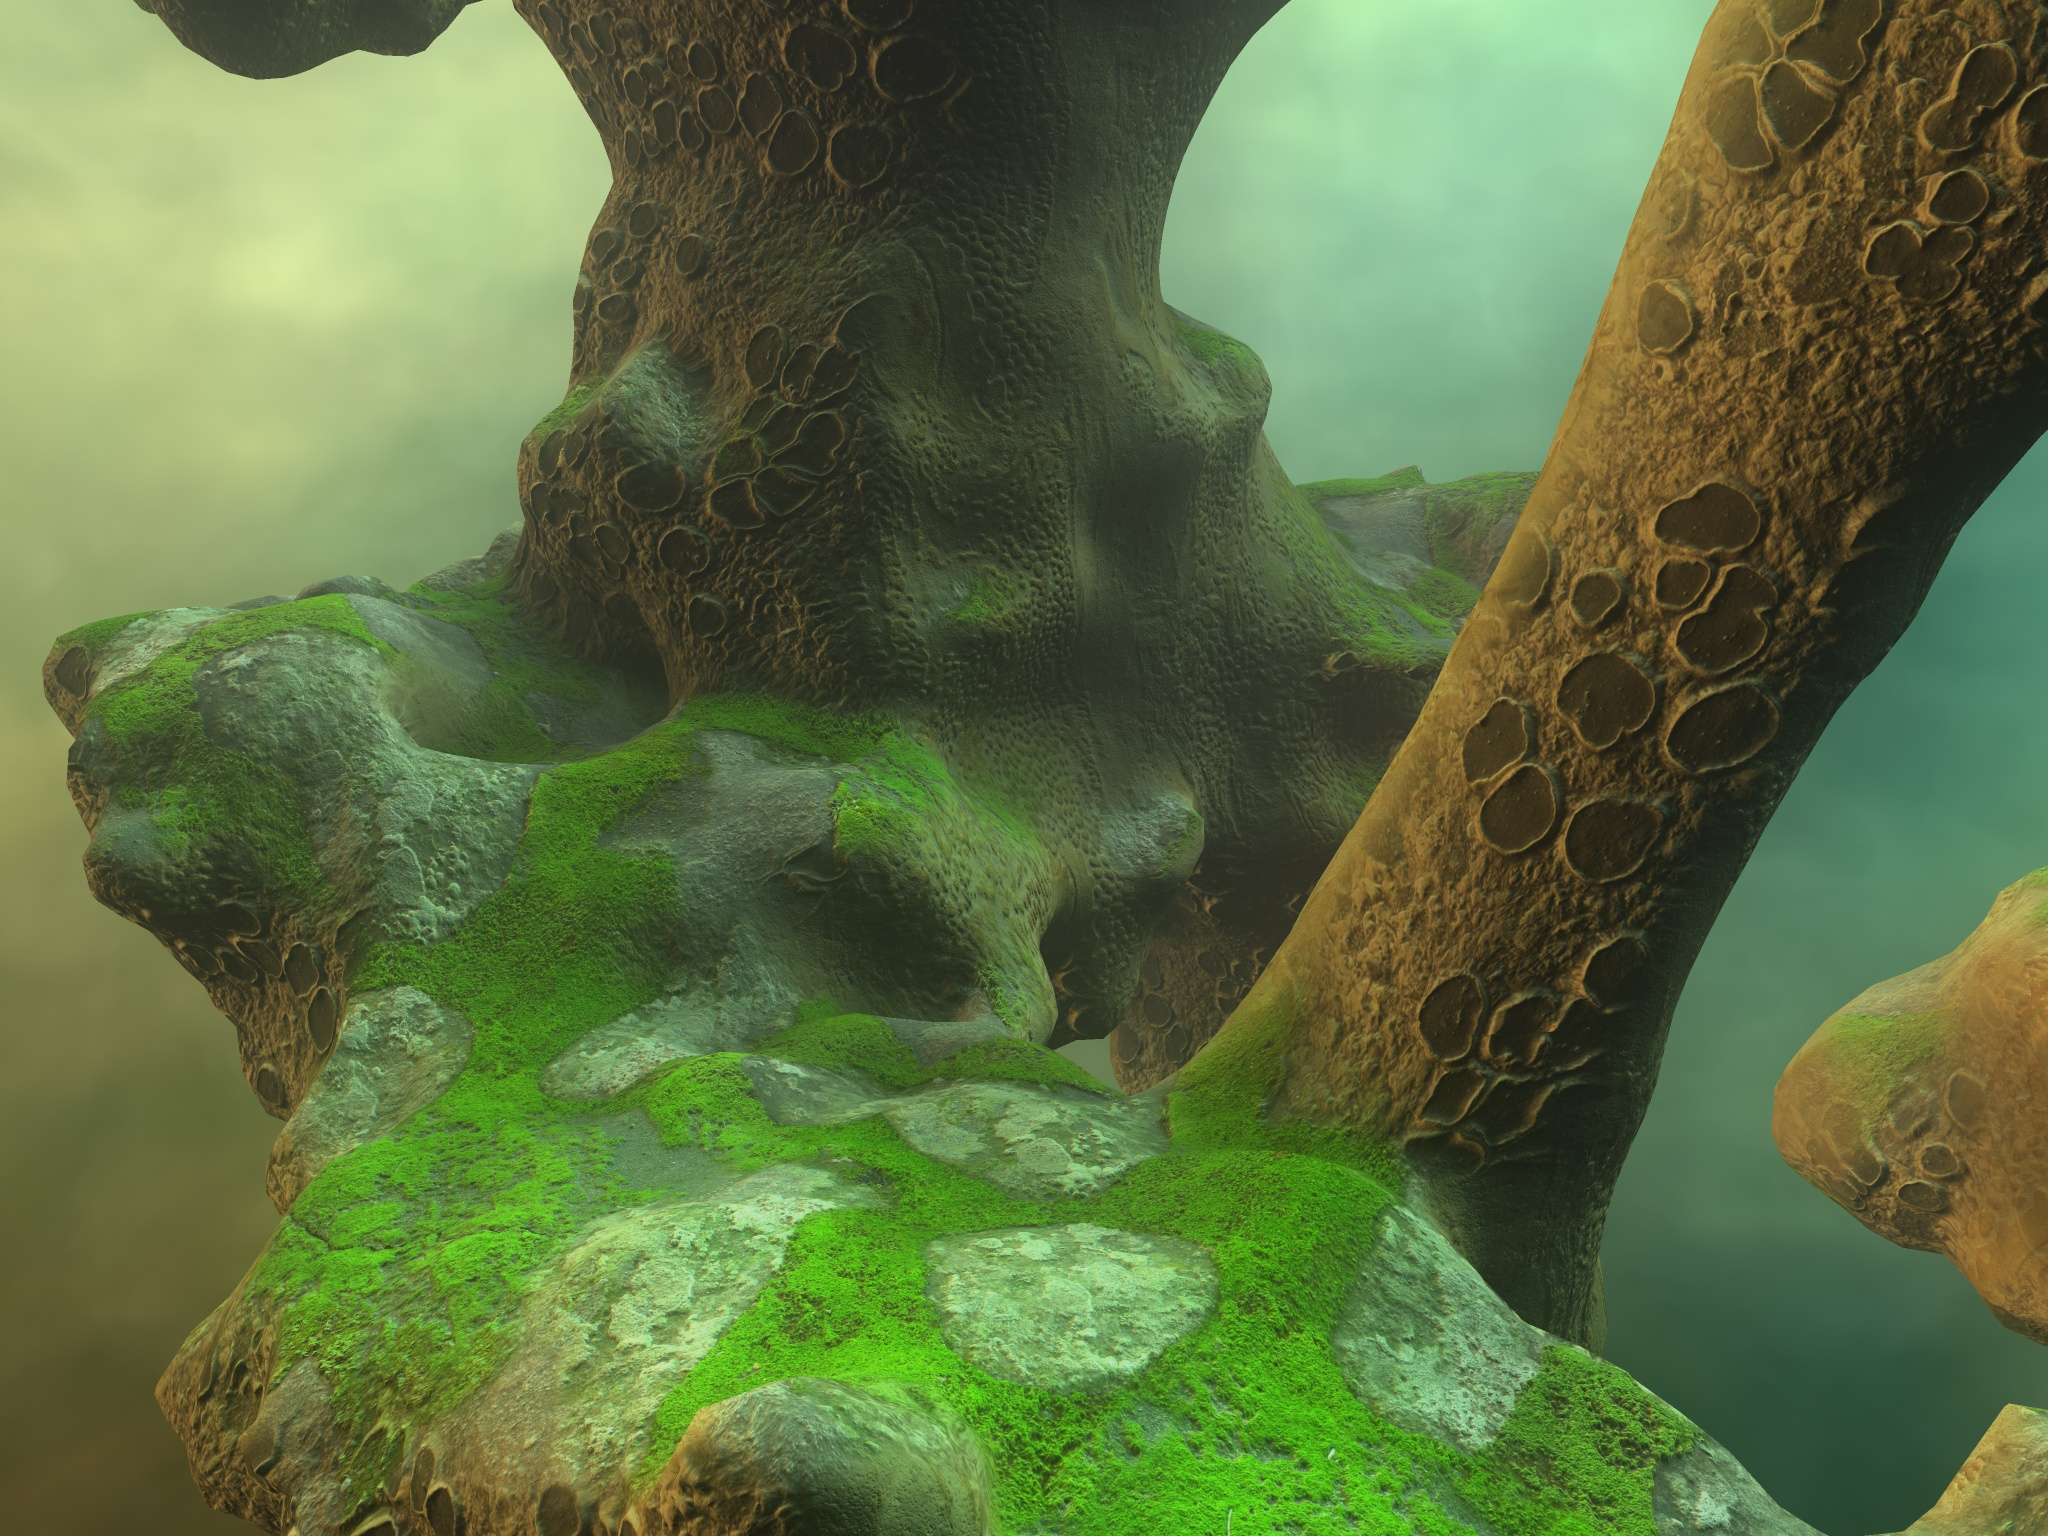
\includegraphics[width=0.5\linewidth]{PICs/cascades}
	\caption{Example of a procedural generated rock. \protect\cite{nvidia::cascades}}\label{cascadesFigure}
\end{figure}

\section{Game Mechanics}
Using PCG as a mechanic requires the player to have control over the kind of content that appears in the game.\cite{pcg::endlessWeb}
\subsection{Current Games}

\subsubsection{Galactic Arms Race}
\todo[inline]{the players’ battle strategies determine the next round of weapons that will be available to them; the creators of the game have shown that there is a large variety in the kinds of weapons players will customize. Because it is a multiplayer game, players can see the different kinds of guns they could have created if they played with different tactics. \protect\cite{pcg::endlessWeb} \protect\cite{pcg::galacticArmsRace}}
\todo[inline]{In GAR, players pilot space ships and fight enemies to acquire unique particle system weapons that are evolved by the game. creates new content in real time through an evolutionary 	algorithm based on the content players liked in the past. a variant of artificial neural network (ANNs), genetically encode and control particle system weapons. That way, during the game, weapon behavior becomes increasingly sophisticated while consistently evolving to suit player tastes. In this way, it is the player rather than the designer who ultimately implicitly determines what kind of content will populate the game. In GAR (figure 2), the goal is to pilot a space ship to defeat enemies, gain experience, earn money, and most importantly, to find advantageous new weapons that are automatically generated by cgNEAT \protect\cite{pcg::galacticArmsRace::evolvingContent}}
\todo[inline]{In GAR (Fig. 4), the goal is to pilot a space ship to defeat enemies, gain experience, earn money, and most importantly, to find advantageous new weapons that are automatically generated by cgNEAT. single-player mode, evolution is directed by the actions of a single player battling NPC aliens in the game, which are controlled by scripted steering behaviors [58] and the boids algorithm [59]. GAR multiplayer evolution is substantially more diverse because the evolutionary population consists of the weapons currently possessed by all players in the game. Players are limited to three weapon slots, each of which holds a single weapon. Destroyed enemies and enemy bases may drop a weapon pickup that contains a novel weapon evolved	by cgNEAT. Players choose in which weapon slot to place the new weapon, but doing so drops the existing weapon in that slot. Thus, players must be selective about which weapons to keep. In this context, an important goal for any game that generates unpredictable content is to indicate what that content will be like before it is taken. To give players an idea of how a	weapon functions before picking it up, weapon pickups emit a miniature particle system preview that behaves exactly as the actual weapon does.\protect\cite{pcg::galacticArmsRace}}

\subsubsection{Inside a Star-Filled Sky}
\todo[inline]{Jason Rohrer’s latest release, Inside a Star-Filled Sky [13] is a good example of a game whose mechanics are PCG-based. ("PCG-Based Game Design - Enabling New Play Experiences through Procedural Content Generation")}
\todo[inline]{Players navigate a space in which they can zoom into or out of recursively nested levels, each one generated from a seed passed from an object in a higher or lower level. Play events that take place on one level of play affect levels above and below themselves. \protect\cite{pcg::endlessWeb}}

\subsubsection{Endless Web}
Is an entirely PCG-based game and thus uses PCG as its core mechanic. It is about fighting the nightmares in human dreams and rescue the trapped one and thus releasing dreamers from their fears. Goal of the game is to rescue six dreamers by exploring the world and make decisions on exploring new areas in the world which affects the parameters of the rescue progress and also the generation of new world parts. For example, if a player kills an enemy then depending on the configuration it strengthens or weakens an associated challenge and furthermore changes the world. \cite{pcg::endlessWeb}
\todo[inline]{Endless Web is fundamentally a game about manipulating a generative space, and the core mechanic involves the player deliberately choosing to influence the generator in different directions through interacting with the glowing tuning portals. This core mechanic is intertwined with the generator; each tuning portal the player interacts with directly changes parameters to the generator. \protect\cite{pcg::endlessWeb}}


\subsubsection{Further Games}
Following games are examples which also use PCG and related mechanics as an important part in their game: Black \& White, Diablo, Dwarf Fortress, Elite, Eve Online, Roque, Spelunky or Minecraft.

\subsection{Possible Core Mechanics}
Quest generation (in "A Prototype Quest Generator Based on a Structural Analysis of Quests from 4 MMORPGs")\\
--> mechanic adaption?
\textbf{Creating New Mechanics and Genres} \cite{pcg::futureOfPcgInGames} \\
Some of the most delightful moments in games come where the game delivers surprising content that follows the theme of what the player has seen previously, such that the player must learn how it works and build new game strategies. For example, new level elements such as platforms where the player controls their movement in New Super Mario Bros (Nintendo EAD 2006). While there has been research in procedurally generating level progressions (Butler et al. 2013), this work uses pre-defined progressions and game elements. How can we create systems that can generate their own progressions? This requires a kind of player modeling that operates at a greater level of detail than numerical scores for enjoyment and frustration, combined with a representation for the mechanics of the game and how game components use them. \cite{pcg::futureOfPcgInGames}\\
\\
\textbf{Multiplayer and Multi-Instance PCG} \cite{pcg::futureOfPcgInGames}\\
What does it mean for multiple players to really engage with generated content, and for a generator to be designed with multiple players in mind? A multiplayer game with multi-instance PCG could have everyone seeing different content while inhabiting the same space, with support for mechanics that allow players to influence each other’s environments. For example, imagine a collaborative multiplayer platforming game where each player’s actions causes new content to be created in another’s, and players must find ways to communicate about how to achieve some common goal. \cite{pcg::futureOfPcgInGames} \\
\\
\textbf{adaptive or player-driven PCG} \cite{pcg::whatIsPCG}\\
Adaptive PCG could have various motivations, such as adjusting the difficulty level of the newly generated content to suit the estimated playing skill of the player, or to generate more content similar to content the player seems to have liked in the past. The timescale at which adaptation occurs could conceivably vary immensely: between games, between levels or even on a second-to-second level \cite{pcg::whatIsPCG}

\subsection{Possible Issues}
Building a PCG-based game instead involves relinquishing direct control over content and treating content generation as a game mechanic. The design of a PCG-based game introduces a number of new design problems, for both the game and the PCG system itself. The design of a PCG-based game introduces a number of new design problems, for both the game and the PCG system itself. Game design issues, from the moment-to-moment pacing of a level to difficulty curves, can no longer be solved through the direct manipulation of game content. The designer must instead design entire ranges of content that can be meaningfully controlled by both the designer and the player. \cite{pcg::endlessWeb}\\
A number of design challenges arose while creating Endless Web from the use of PCG as the core mechanic. The primary challenge came in determining how to balance this control over the generator between the player and the designer, so that the player makes meaningful decisions but all of those decisions lead to an engaging, designed experience. Other design problems include teaching the player to explore a generative space, providing well-placed goals to encourage this exploration, and art and audio issues that arose from having no knowledge at design time of how levels would be structured during play.  \cite{pcg::endlessWeb}
\subsection{Summary}

%
% ------------------------------- NEW CHAPTER ------------------------------- %
%
\clearpage
\chapter{\acl{ML}}

\section{Theoretical Introduction}
Theory of PCG and ML in general.

\subsection{Regression}
\subsection{Classification}
\subsection{Clustering}
\subsection{Reinforcement Learning}

\section{Learning Models}
Which training models are used in ML? --> the 5 tribes of ML
\subsection{Linear}
\subsection{K-Nearest Neighbor}
\subsection{Decision Tree}
\subsection{\acl{SVM}}
\subsection{Neural Networks}
\subsubsection{\acl{ANN}}
\subsubsection{\acl{CNN}}

\section{Use Cases}
\subsection{Data Science}
stick to game related stuff, like alpha go
\subsection{Games}
\todo[inline]{The most common application of machine learning is to optimize the policy that controls non-player characters (NPCs). For example, the ANN race car controllers Colin McRae Rally 2.0 and Forza Motorsport 2 and the creature brains in Creatures 3 and Black and White 2 are learned. \protect\cite{pcg::galacticArmsRace::evolvingContent}}
\subsubsection{Examples}
\subsubsection{Possibilities}

\section{Development}
How to use PCG and ML in a game engine? What are some of the best practices and approaches for using PCG and ML in a game?

\subsection{Conceptual Implementation}
Basic sample PCG and ML implementations in a game engine.

\subsection{Possible Issues}
Issues of PCG and ML in games and game engines.


\section{Game Mechanics}
\subsection{Current Games}
\subsection{Possible Mechanics}
\subsection{Summary}


%
% ------------------------------- NEW CHAPTER ------------------------------- %
%
\clearpage
\chapter{\acl{PCGML}}
\section{What is it About?}
Theory of PCGML and its methods in general.
Evaluation of PCGML hardware and software requirements
\section{Current Use in Games}
\section{Possibilities}
\section{Difference to Usual \acl{PCG}}
\section{Example Implementations}
Theory of PCGML and its methods in general.
\section{Learning Models}
Comparison of PCGML learning models
\subsection{Markov Chains}
\subsection{\acl{ANN}}
\subsection{Bayes}
look for a paper of "Guzdial"
\section{In a Game Engine}
research on different PCGML implementations and practical usage possibilities in a game engine
\subsection{Conceptual Prototype}
\subsection{Possible Issues}
%
% ------------------------------- NEW CHAPTER ------------------------------- %
%
\clearpage
\chapter{\acl{PCGML} Game Mechanics}
the design process for \cite{pcg::endlessWeb} followed the principles of \cite{ai::gameDesign} with Launchpad as the AI system.

\section{First Considerations}

\section{Possibilities}
maybe read over \cite{pcg::endlessWeb} again\\
Concepts of possible PCGML game mechanics.

\subsection{Role-Model}
A \ac{PCGML} system replicates content which is generated by players of various levels of skill or generates content suitable for players of certain skill levels. New players are trained by replicating the content or by playing the generated content in the form of generative tutorial. \cite{pcgml::paper}

\subsection{Trainee}
The player trains a \ac{PCGML} system to generate a piece of necessary content (e.g., part of a puzzle or level geometry). \cite{pcgml::paper}

\subsection{Editable}
Rather than training the AI to generate the missing puzzle piece via examples, the player changes the internal model’s values until acceptable content is generated. \cite{pcgml::paper}

\subsection{Guided}
The player corrects the \ac{PCG} system’s output to fulfil increasingly difficult requirements. The \ac{AI}, in turn, learns from the player’s corrections, following the player’s guidance. \cite{pcgml::paper}

\subsection{Co-Creator}
The player and a \ac{PCGML} system take turns in creating content, moving towards some external requirements. The \ac{PCGML} system learns from the player’s examples. \cite{pcgml::paper} 

\subsection{Adversary}
The player produces content that the \ac{PCGML} system must replicate by generation to survive or vice versa in a “call and response” battle. \cite{pcgml::paper}

\subsection{Spectacle}
The \ac{PCGML} system is trained to replicate patterns that are sensorically impressive or cognitively interesting. \cite{pcgml::paper}

\section{Conceptual Prototypes (with evaluation)}
A test implementation of PCGML game mechanics in a game engine.

\subsection{Comparison of Different Mechanics}
Comparison of implemented PCGML game mechanics prototypes.

\section{Summary}
what is the best game mechanic? why? etc
%
% ------------------------------- NEW CHAPTER ------------------------------- %
%
\clearpage
\chapter{Game Prototype}
Development of a game with one of the best-evaluated PCGML game mechanic as the central game mechanic of the game.
\section{Considerations}

\subsection{Which Game Engine?}
There are 2 main engines which are commonly used thorough the industry due to their fact of free to use.

\section{Game Design}
\textbf{Designing Awesome AI for Games - Summary (GDC Talk)}
\begin{enumerate}
	\item Support the core experience
	\item Watch people play and get in their heads
	\item Identify broad behaviours
	\item Start simple
	\item Figure out what the brain gives you for free
	\item Try going simpler before you go complex
\end{enumerate}

\section{Implementation}
\subsection{Technical Approach}
Classes, Diagrams, why use what - eg. why use neural network over other and stuff like that!
\subsection{Online or Offline?}
\section{Performance Measurements}
\subsection{Improvement Iterations}
\section{Playtest}
\subsection{Preparations}
\subsection{Evaluation}
Evaluation of playtesters feedback.
\section{Result}
show the fucking game and the mechanics!

%
% ------------------------------- NEW CHAPTER ------------------------------- %
%
\clearpage
\chapter{Conclusion}
The meaning of the use of PCGML as a game mechanic for the future of games and gaming. 
\section{Summary}
\section{Research Result}
\section{Future Work}
%
% Hier beginnen die Verzeichnisse.
%
\clearpage
\ifthenelse{\equal{\FHTWCitationType}{HARVARD}}{}{\bibliographystyle{gerabbrv}}
\bibliography{Literatur}
\clearpage

% Das Abbildungsverzeichnis
\listoffigures
\clearpage

% Das Tabellenverzeichnis
\listoftables
\clearpage

% Das Quellcodeverzeichnis
\listofcode
\clearpage

\phantomsection
\addcontentsline{toc}{chapter}{\listacroname}
\chapter*{\listacroname}
\begin{acronym}[XXXXX]
	\acro{2D}{2-Dimensional}
	\acro{3D}{3-Dimensional}
	\acro{AI}{Artificial Intelligence}
	\acro{ANN}{Artificial Neural Network}
	\acro{CNN}{Convolutional Neural Network}
	\acro{GB}{Gigabyte}
	\acro{MDA}{Mechanics-Dynamics-Aesthetics}
	\acro{ML}{Machine Learning}
	\acro{PC}{Personal Computer}
    \acro{PCG}{Procedural Content Generation}
    \acro{PCGML}{Procedural Content Generation via Machine Learning}
    %\acro{RPG}{Roleplay Game}
    \acro{RNG}{Random Number Generator}
    \acro{SVM}{Support Vector Machine}
\end{acronym}

%
% Hier beginnt der Anhang.
%
\clearpage
\appendix
%\chapter{Appendix A}
\end{document}